\documentclass[final,leqno,onefignum,onetabnum]{siamltex1213}

%  typeset with TeX and DVI
\usepackage{amsmath,amssymb}
\usepackage{rotating}
%\usepackage[dvips]{graphicx}
%\usepackage[]{epsfig}
%\usepackage[]{pdflatex}
\usepackage{overpic}
\usepackage{tikz}


\newcommand{\pathname}{common/}
\newcommand{\fullpath}{\pathname}

\input{\pathname declarations.tex}

% SIAM Journal on APPLIED MATHEMATICS
\title{Scalar fields and limbic measurements\\ over the unit disk \thanks{This work was
supported by the Society for Industrial and Applied Mathematics}} 

%\author{Daniel Topa, James Cooley, and Pedro Embid.\thanks{Los Alamos National Laboratory 
%(\email{dantopa@lanl.gov}). Questions, comments, or corrections
%to this document may be directed to that email address.}}
\author{D.~M. Topa\footnotemark[1]\ \footnotemark[2] \and P.~F. Embid\footnotemark[1] \and J.~H. Cooley\footnotemark[1]}

\footnotetext[1]{Los Alamos National Laboratory, Los Alamos New Mexico 87545}
\footnotetext[2]{Department of Mathematics and Statistics, University of New Mexico, Albuquerque New Mexico 87131}

\begin{document}
\maketitle
\slugger{siap}{xxxx}{xx}{x}{x--x}%slugger should be set to mms, siap, sicomp, sicon, sidma, sima, simax, sinum, siopt, sisc, or sirev

\begin{abstract}
The goals of this paper are to present basic mathematical tools for the analysis of scalar fields over the unit disk. In particular, we discuss limbic measurements in the continuum limit and for spatially extended sources and detectors. The physical motivation is x-ray spectroscopy of spheres under radiative compression and as such this work is covers mathematical preliminaries for a 2-D approximation in advance of a complete 3-D analysis.
\end{abstract}

\begin{keywords}
 Radiative transport, Zernike polynomials, limbic measurement
\end{keywords}

\begin{AMS}
15-02, 33E-02
\end{AMS}


\pagestyle{myheadings}
\thispagestyle{plain}
\markboth{DANIEL TOPA, PEDRO EMBID, AND JAMES COOLEY}{SCALAR FIELDS AND LIMBIC MEASUREMENTS OVER THE UNIT DISK}

%     S   S   S   S   S   S   S   S   S   S   S   S   S   S   S   S   S   S   S   S
\section{Introduction}

Our physical motivation is to study radiative implosion of spherical capsules of isotopic hydrogen. Such experiments are the staple at facilities like the National Ignition Facility and the Omega Laser Facility. Typical capsules are tiny with a radius of one to two millimeters. They are pressurized at 10 to 15 atmospheres. They may be cryogenically cooled or at room temperature. They often contain a mix of deuterium, D, and tritium, T.

To help focus the analysis, we assume the capsules are compressed uniformly by a bath of high energy x-rays. We assume the outer shell of the capsule is ablated creating an inward compression due to the rocket effect \cite{Lindle}. We are interested in cases where the capsule shell is sturdy enough to support uniform compression; that is, the capsule boundary remains spherical until maximum compression is reached (bang time). One valuable diagnostic is a dopant which produces a bright x-ray source in the temperature and pressure ranges of interest. For example, this may be a smattering of argon gas inside the capsule or titanium dopant in the outer shell. The measurement of interest is the intensities for the two dominant x-ray lines. 

The detectors which record these intensities resolve the capsule into 5--25 radial zones. There are detectors on three spatial axes to allow three-dimensional imaging of the capsule. While our ultimate goal is to study phenomena like the Rayleigh-Taylor instability which shatter spherical symmetries, we are interested in developing foundation tools which use intensity measurements to divine thermodynamic profiles inside the capsule. This motivates an initial consideration of spherical symmetry.

\clearpage

%     S   S   S   S   S   S   S   S   S   S   S   S   S   S   S   S   S   S   S   S
\section{Radiative transport}
For the problem at hand the data is a spatially resolved set of $x$-ray intensity measurements. A dopant in the device is selected to create a known signature over a temperature and pressure regime of interest. We rely upon this signature to resolve the thermodynamic profiles in the capsule.The mathematical challenge before us is to use the intensity measurements and the radiative transport equation to divine the physics inside the capsule.

Consider a photon packet within the capsule. Between creation and detection we will consider three mathematically distinct phenomena: absorption, emission and scattering.

We treat the radiative transport equation as a one-dimensional integro-differential equation of the form $Lu(r,\mu)=f(r)$
  % % % EQUATION
  \begin{equation}
   \paren{ \mu \pd{}{r} + \frac{1-\mu^{2}}{r} \pd{}{\mu} + k(r)} I(r,\mu) + \scat \\
    = -k(r) J(r)
  \label{eq:intensity transport}
  \end{equation}
  % %
For comparison, see Hummer\cite{Hummer}.

The archetype ODE for radiative transport is
  % % % EQUATION
  \begin{equation}
    I'(s) + I(s) = 1
  \end{equation}
  % % %
which is a decay equations with a forcing term.
  % % % EQUATION
  \begin{equation}
    I(r) = e^{-\int_{r}^{1} \alpha(r')dr'} \paren{ 1 - \int_{r}^{1} e^{\int_{r'}^{1}\alpha(r')dr'} j(r'')dr''}
  \end{equation}
  % % %


%    SS  SS  SS  SS  SS  SS  SS  SS  SS  SS  SS  SS  SS  SS  SS  SS  SS  SS  SS  SS
\subsection{Closing}
In our application we enjoy the benefit of having functional forms for the absorption $\alpha(T,\rho)$ and emission $j(T,\rho)$.

The long range goal is to find 3D solutions of the form $\psi(r,\theta,\phi)$ using a scattering kernel. But there are mathematical preliminaries to address.

In this treatment we avoid the necessary evil of units for two reasons. First, the measurement is 

The mathematical problem distills to this: given an intensity profile $\pr$ and the maps $\alpha(T,\rho)$ and $j(T,\rho)$ find the thermodynamic profile $T(r)$ and and $\rho(r)$ inside the capsule assuming the validity of the radiative transport equation.

\begin{enumerate}
  %
  \item{Compute opacity map $\alpha(T,\rho)$ and emissivity map $j(T,\rho)$.}
  %
  \item{Use detector measurements to find the integrated intensity $\ii$.}
  %
  \item{Construct $\alpha(r)$ and $j(r)$.}
  %
  \item{Compute thermodynamic profiles $T(r)$ and $\rho(r)$.}
  %
\end{enumerate}

%\clearpage

%     S   S   S   S   S   S   S   S   S   S   S   S   S   S   S   S   S   S   S   S
\section{Polynomial basis}

Of interest are spherically symmetric functions $\psi\colon \real{2} \mapsto \real{}$. We require functions square-integrable over the unit disk $L_{2}(\dtwo)$. The two most common polynomial sets are the one posed by Zernike \cite{Zernike} and the other proposed by Bhatia and Wolf \cite{Bhatia}. Both sets are discussed briefly in the appendix. For either case, we are interested in a rotationally invariant subset where the angular frequency $m=0$.

%    SS  SS  SS  SS  SS  SS  SS  SS  SS  SS  SS  SS  SS  SS  SS  SS  SS  SS  SS  SS
\subsection{Polynomial basis}  %  +  +  +  +  +  +  +  +  +  +
We choose the set of Zernike because of the order-by-order correspondence to the Seidel aberrations and we adopt Zernike's convention
  % % % EQUATION
  \begin{equation}
    V_{n}^{m} (r, \theta ) = R_{n}^{m}(r) e^{i m \theta}
    \label{eq:Zernike separation}
  \end{equation}
  % % %
where $n$ and $m$ are positive integers such that $n-m$ is a positive, even number. The order is $n$, the angular frequency is $m$. The radial functions are defined in  the appendix. The full set 
$$\lst{V_{0}^{0} (r, \theta ),\, V_{1}^{1} (r, \theta ),\, V_{2}^{0} (r, \theta ),\, V_{2}^{2} (r, \theta ),\, \dots}$$ 
is complete\cite{complete} over the unit disk and this allows for the uniform approximation of continuous.
  % % % EQUATION
  \begin{equation}
    \prt = \sum_{n=0}^{d} \sum_{m=\odot}^{n(2)} \alpha_{n,m} R_{n}^{m}(r) e^{i m \theta}, \qquad \alpha \in \cmplx{\half d (d+1)}
    \label{eq:Zernike expansion}
  \end{equation}
  % % %
The degree of the fit is $d=0,1,2,\dots$ The sum over $m$ runs from $\odot=n\bmod 2$ to $n$ in increments of 2. For example, when the order $n=4$ the angular velocity takes the values $m=0,2,4$; for $n=5$ we have $m=1,3,5$.

Eventually we need to consider fields like $\prt$ with angular dependence. The first stage of this analysis is restricted to radially symmetric fields $\pr$ which restricts us to the subset of the Zernike polynomials with radial symmetry. This is set with angular frequency $m=0$.

One must establish that the completeness of the culled set with $m=0$ is dense in the space of continuous, rotationally invariant functions with respect to the uniform norm. This task is simplified by Trent's extension  \cite{Trent} of the \ms theorem to the closed unit disk. Consider the space $L_{2}(\dtwo)$ and let $S$ be the span of the set of monomials of even powers $\lst{1,r^{2},r^{4},\dots}$.\footnote{We define $\lim\limits_{r\to0}r^{0}\equiv0$.} The closure of $S$ is the set $\Sbar$ which represents the rotationally invariant elements which can be approximated by polynomials. In this case $\Sbar \subseteq L_{2}(\dtwo)$. The following theorem connects the reduced Zernike polynomials and the even monomials.

\input{sections/basis/"thm completeness"}  %  <  <  <  <  <  <  <  <  <

The reduced polynomial set for $m=0$ is previewed in figure \eqref{fig:cutaways} as two subsets, a presentation which reminds us that the individual sequences for $k$ even and $k$ odd are Cauchy. These two sequences are further distinguished by their behavior at $r=1/\sqrt{2}$. Given $k=0,1,2,\dots$,
\begin{equation}
  \begin{split}
    R_{2(2k)}^{0}\paren{ 1/\sqrt{2} } &= 0 , \\
    \td{}{r}R_{2(2k+1)}^{0}\paren{ 1/\sqrt{2} } &= 0 .
  \end{split}
\end{equation}

%  figure placement: here, top, bottom, or page    ><  ><  ><  ><  ><  ><
\begin{figure}[htbp] 
   \centering
   \includegraphics[ width = 5in ]{graphics/parity_pts_00500_F.eps} 
   \caption{Function sequences for the angular velocity $m=0$ subset grouped by parity and shown in cutaway: $\lst{Z_{2(2k)}^{0}(r,\theta)}_{k=0}^{3}$ (top), and $\lst{Z_{2(2k+1)}^{0}(r,\theta)}_{k=0}^{3}$ (bottom). The Fourier like nature of these polynomials is apparent; the top row functions like cosine terms, the bottom like sine terms. }
   \label{fig:cutaways}
\end{figure}
%
These polynomials are used to represent rotationally invariant scalar fields over the unit disk. Let $n$ be the highest order term in the sequence, the expansion is cast with amplitudes $\alpha$:
%
\begin{equation}
  \pr = \alpha_{0} + \alpha_{2}R_{2}^{0}(r) + \alpha_{4}R_{4}^{0}(r) + \dots + \alpha_{n}R_{n}^{0}(r) = \sum_{k=0}^{d}\alpha_{2k}R_{2k}^{0}(r)
  \label{eq:Zernike alpha}
\end{equation}
The summation control parameter $d=n/2$.
The scalar field $\pr$ represents measurable scalars such as intensity, temperature or density.
%
The orthogonality of the Zernike polynomial set is a useful property (as seen in the following theorem \eqref{thm:completeness} and \cite{Topa}). Yet the linear independence of this set is most often the property to exploit as in theorem \eqref{thm:completeness}. The reason for this is two fold. 

First, Zernike's polynomials are constructed to be in an order-by-order correspondence with the optical aberrations popularized by Seidel \cite{Zernike}. This empowers exact affine transformations between the representations of Zernike and Seidel. Secondly, orthogonality is predicated upon the domain and the topology. The Zernike polynomials are orthogonal over $\spaceL$ but not upon $\spacel$. Since measurements are inherently finite objects and computer algorithms are built upon discrete meshes we are excluded from using orthogonality\footnote{Codes built upon orthogonality extend computation time; for a mesh of $N$ points the error in the accuracy is $\Order{N}$. Zernike expansion amplitudes are no longer independent and cannot be calculate linearly. This demands the solution of a full rank linear system  \cite{Topa orthogonality}.} and rely instead upon linear independence. We are thus compelled to built our approximation upon the minimal spanning set, the monomials:
%
\begin{equation}
  \pr = a_{0} + a_{2}r^{2} + a_{4}r^{4} + \dots + a_{n}r^{n} = \sum_{k=0}^{d} a_{2k}r^{2k}
  \label{eq:even polynomials}
\end{equation}
%
A simple change of basis toggles the coordinates $\alpha$ in the Zernike basis and the coordinates $a$ in the monomial basis:
%%%
\begin{equation}
  \alpha = \brac{T}_{Zernike}^{-1} a.
\end{equation}
%%%
The three lowest Zernike polynomials have the monomial representation $R_{0}^{0}(r) = 0$, $R_{0}^{0}(r) = 2r^{2} - 1$ and  $R_{6}^{0}(r) = 6r^{4} - 6r^{2} + 1$, the change of basis matrix is
%%%
\begin{equation}
  \brac{T}_{Zernike}^{-1} = \mat{rrr}{
  1 & -1 &  1 \\
  0 &  2 & -6 \\
  0 &  0 &  6 }^{-1}
\end{equation}
%%%

Very much like a Fourier decomposition, the Zernike composition describes zero mean oscillations about a constant value given by the order $n=0$ amplitude. This is not apparent given the polynomial weighting in the Zernike terms seen in \eqref{eq:Zernike separation}. However, the following proof verifies the contention. (The proof is trivially extended to include $m=1,2,\dots$)

\input{sections/basis/"thm zero mean"}  %  <  <  <  <  <  <  <  <  <

The immediate advantage is that the Zernike decompositions automatically provide for mean values including valuable thermodynamic properties such as temperature and pressure.

%    SS  SS  SS  SS  SS  SS  SS  SS  SS  SS  SS  SS  SS  SS  SS  SS  SS  SS  SS  SS
\subsection{Trajectories}
With the scalar fields being represented by a Zernike expansion, These are generalized Lissajous figures.
%  figure placement: here, top, bottom, or page    ><  ><  ><  ><  ><  ><  ><  ><  ><  ><  ><  ><  ><  ><  ><  ><  ><  ><
\begin{figure}[htbp] 
   \centering
   \includegraphics[ width = 2.25in ]{graphics/lissajous__04_10.eps} \qquad 
   \includegraphics[ width = 2.25in ]{graphics/lissajous__10_20.eps} \\[5pt]
   $R_{4}^{0}(r) \times R_{10}^{0}(r)$ \qquad \qquad \qquad \qquad \qquad $R_{10}^{0}(r) \times R_{20}^{0}(r)$
   \caption{Generalized Lissajous figures using the ideal gas law \eqref{eq:ideal} for the equation of state. }
   \label{fig:lissajous}
\end{figure}

%     S   S   S   S   S   S   S   S   S   S   S   S   S   S   S   S   S   S   S   S
\section{Limbic measurement}
In experimental measurements of interest (such as those at NIF and the Omega Laser Facility) the detector array is in the plane of the unit disk and views a portion of the disk over the range $-\pi/2 \le \phi \le \pi/2$. The angle is defined on the disk and the ray at $\phi = 0$ intersects the detector array at a right angle. What the detectors record in the $x$-ray intensity integrated along a limbic path. We now discuss the geometry of these paths.

\subsection{Infinitesimal detectors (Continuum case)}
We start with the idealization of infinitesimal detectors. Basic detector geometry is shown in figure \eqref{fig:continuum} where the detector plane represents a continuum of detectors. These detectors record a response function $Y(b)$ where $b$ is the impact parameter, an offset from the ray at $\phi = 0$. Handling this offset requires some attention.

%  figure placement: here, top, bottom, or page    ><  ><  ><  ><  ><  ><  ><  ><  ><  ><  ><  ><  ><  ><  ><  ><  ><  ><
\begin{figure}[htbp] 
   \centering
   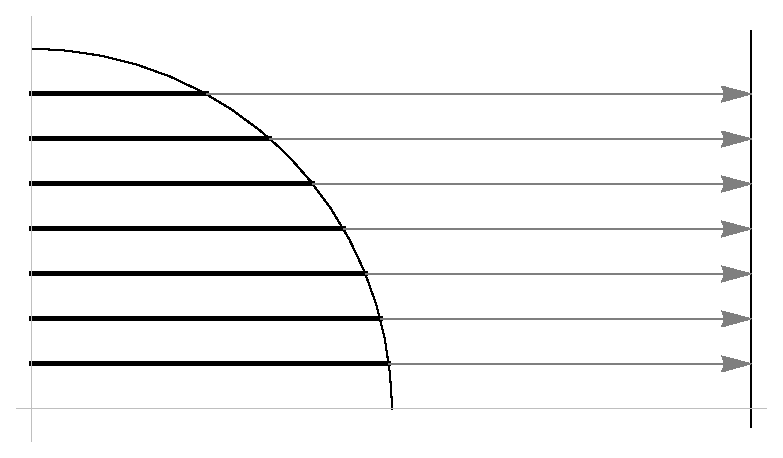
\includegraphics[ width = 2.5in ]{graphics/continuum.eps} 
   \caption{Basic detector geometry. The quarter capsule is shown on the left, the detectors as a plane on the right. The dark lines represent packets of $x-$rays traveling through and interacting with the capsule. Because of an imaging system, the detectors see the intensity at the surface of the capsule which is transported to the detectors. The line of site is characterized by an impact parameter $b$ measuring distance from the equator. Our discussion first considers the case where $b$ is a continuous variable $0\le b \le 1$, from the equator to the apex.}
   \label{fig:continuum}
\end{figure}

While we are trying to discern $\psi(r)$ a scalar field as a function of distance from the origin, we record the integral of an intensity function along the limbic paths in figure \eqref{fig:continuum}. Let $\gamma_{b}$ represent one such path as seen in figure \eqref{fig:gamma}. The detector at $b$ measures the intensity at the surface of the capsule; the measurement is the response function $Y(b)$.

%  figure placement: here, top, bottom, or page    ><  ><  ><  ><  ><  ><  ><  ><  ><  ><  ><  ><  ><  ><  ><  ><  ><  ><
\begin{figure}[htbp] 
   \centering
   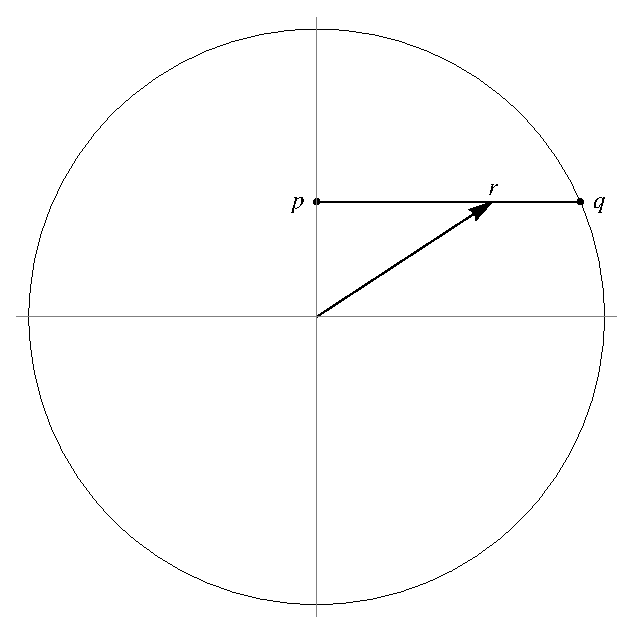
\includegraphics[ width = 2.5in ]{graphics/line_integral.eps} 
   \caption{The line integral in figure \eqref{fig:continuum}. The path $\gamma_{b}$ is the convex set connecting $p$ to $q$. The magnitude of the vector $r$ is given as a function of the parameter $b$.}
   \label{fig:gamma}
\end{figure}
%

%   SSS SSS SSS SSS SSS SSS SSS SSS SSS SSS SSS SSS SSS SSS SSS SSS SSS SSS SSS SSS
\subsubsection{Response function}
The response function is an integral along the limbic path characterized by an impact parameter $b$:
%
\begin{equation}
  Y(b) = \int_{\gamma_{b}} \psi(s) ds .
  \label{eq:response}
\end{equation}
%
The measurement represents the strength of the photon packet exiting the capsule. These photons encode thermodynamic information along the the path $\gamma_{b}$. This path is the convex set connecting $p = \mat{c}{b\\0}$ to $q = \mat{c}{b\\\cost}$:
  % % % EQUATION
  \begin{equation}
    \gamma_{b}(t) = p (1-t) + q t, \qquad 0 \le t \le 1.
  \end{equation}
  % % %
This formulation establishes convexity. 

To parameterize the function $\psi$ along this line given by $0\le x_{1} \le \cost$, $x_{2} = b$ define the radial distance $r$ in figure \eqref{fig:gamma} as
  % % % EQUATION
  \begin{equation}
    r = \xpbs
  \end{equation}
  % % %
then the integral in \eqref{eq:response} becomes
  % % % EQUATION
  \begin{equation}
    \begin{split}
      Y(b) &= \int_{0}^{\cost} \psi \paren{\xpbs} dx_{1}, \qquad b \in [0,1] \\
           &= \int_{0}^{\cost} \paren{ a_{0}\paren{\xpbs}^{0} + a_{2}\paren{\xpbs}^{2} + a_{4}\paren{\xpbs}^{4} + \cdots } dx_{1}
    \end{split}
    \label{eq:response modes}
  \end{equation}
  % % %
%Discussion of existence and uniqueness is deferred to section \S \eqref{ssec:extended}.
For $k=0,1,2,\dots$ the integrals in \eqref{eq:response modes} is
  % % % EQUATION
  \begin{multline}
    \int_{0}^{\cost} \paren{\xpbs}^{2k} dx_{1} = \paren{2b^{2} \cost (k+1)}^{-1} \times\\
    \paren{\hg{1}{k+\frac{3}{2}}{-\half}{1-\frac{1}{b^{2}}} + \paren{2b^{2}(k+2)-2k-5}\hg{1}{k+\frac{3}{2}}{\half}{1-\frac{1}{b^{2}}}} .
  \label{eq:hg 1}
  \end{multline}
  % % %
%
For $\abs{z}>1$ and $a-b\notin\mathbb{Z}$ the hypergeometric series is defined\footnote{Wolfram Functions Site,\\ \texttt{http://functions.wolfram.com/HypergeometricFunctions/Hypergeometric2F1/02/02/}.} as
%
\begin{multline}
  \hg{a}{b}{c}{z} = 
    \frac{\Gamma(b-a)\Gamma(c)\paren{-r}^{-a}} {\Gamma(b)\Gamma(c-a)}
      \sum_{k=0}^{\infty} \frac{(a)_{k}(a-c+1)_{k}z^{-k}} {k!(a-b+1)_{k}} \\ +
    \frac{\Gamma(a-b)\Gamma(c)\paren{-r}^{-b}} {\Gamma(a)\Gamma(c-b)}
      \sum_{k=0}^{\infty} \frac{(b)_{k}(b-c+1)_{k}z^{-k}} {k!(a-b+1)_{k}}
  \label{eq:hypergeometric}
\end{multline}
%
and the rising Pochhammer symbol is 
%
\begin{equation}
  (a)_{n} = 
  \begin{cases}
    1 & n=0 \\
    a(a+1)\cdots(a+n-1) & n > 0
  \end{cases}
\end{equation}
%
For this problem the arguments of the Pochhammer function are natural numbers and we may use this definition:\footnote{NIST Digital Library of Mathematical Functions, \texttt{http://dlmf.nist.gov/5.2}.}
  % - -  e q u a t i o n
  \begin{equation}
     (a)_{n} = \frac{\Gamma(a+n)} {\Gamma(n)}.
  \end{equation}
  % - -
Equation \eqref{eq:hypergeometric} tames the unbounded growth of the $1/b^{2}$ term in the function argument. 

The modes in the expansion \eqref{eq:even polynomials} imprint upon \eqref{eq:response modes} motivating the need to resolve the response function\footnote{To avoid the ambiguous form $0^{0}$, we define the iterated limit in the response function as $\lim_{r\to0,n\to0}r^{n}\equiv 1$.} into modes:
%
\begin{equation}
  \begin{split}
%
    \mathcal{Y}_{0} (b) =
    \int_{0}^{\cost} \paren{ \xpbs }^{0} dx_{1} &=
      \cost \\
%
    \mathcal{Y}_{2} (b) =
    \int_{0}^{\cost} \paren{ \xpbs }^{2} dx_{1} &=
      \frac{1}{3} \paren{ 1 + 2b^{2} } \cost \\
%
    \mathcal{Y}_{4} (b) =
    \int_{0}^{\cost} \paren{ \xpbs }^{4} dx_{1} &=
      \frac{1}{15} \paren{ 3 + 4b^{2} + 8b^{4} } \cost \\
     & \phantom{a}\vdots
%
%    Y_{6} (b) =
%    \int_{0}^{\cost} \paren{ \xpbs }^{6} dx_{1} &=
%      \frac{1}{35} \paren{ 5 + 6b^{2} + 8b^{4} + 16b^{6} } \cost \\
  \end{split}
  \label{eq:family Y}
\end{equation}
%
The approximation in \eqref{eq:response modes} takes the form
  % = =  e q u a t i o n
  \begin{equation}
    Y(b) \approx a_{0}\mathcal{Y}_{0} (b) + a_{2}\mathcal{Y}_{2} (b) + a_{4}\mathcal{Y}_{4} (b) + \dots
  \label{eq:mathcal Y}
  \end{equation}
  % = =
The response functions $\mathcal{Y}$ can be assembled using recursion as seen the in following lemma.
%
%Define the response polynomials as
%\begin{equation}
%  \begin{split}
%    \mathcal{R}_{0}(b) &= 1, \\
%    \mathcal{R}_{2}(b) &= \frac{1}{3} \paren{ 1 + 2b^{2} }, \\
%    \mathcal{R}_{4}(b) &= \frac{1}{15} \paren{ 3 + 4b^{2} + 8b^{4} }, \\
%    \mathcal{R}_{6}(b) &= \frac{1}{35} \paren{ 5 + 6b^{2} + 8b^{4} + 16b^{6} }, \dots \\
%  \end{split}
%\end{equation}
%  are able to
\input{sections/limbic/"thm recursion"}  %  <  <  <  <  <  <  <  <  <  <
The polynomic portion of the sequence $\mathcal{Y}$ 
%%%
\begin{equation}
  \lst{1, \frac{1}{3}\paren{ 1 + 2b^{2} }, \frac{1}{15}\paren{ 3 + 4b^{2} + 8b^{2} }, \frac{1}{35} \paren{ 5 + 6b^{2} + 8b^{4} + 16b^{6}, \dots } }
  \label{eq:bowls}
\end{equation}
%%%
is a series of bowl functions as seen in figure \ref{fig:bowls}. This figure suggests that we can expect problems resolving data near the apex of the capsule where $b=1$.
\begin{figure}[htbp] %  figure placement: here, top, bottom, or page
   \centering
   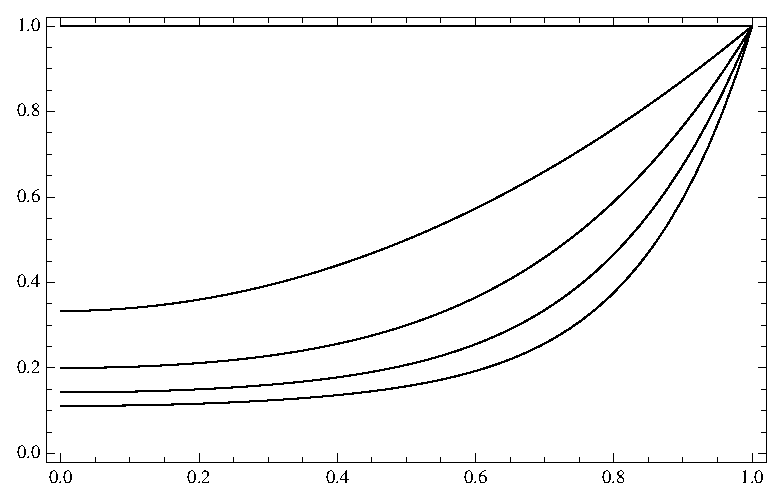
\includegraphics[ width = 4in ]{graphics/bowls.eps} 
   \caption{The sequence of bowl functions in \eqref{eq:bowls}.}
   \label{fig:bowls}
\end{figure}

The lowest modes $\mathcal{Y}$ are displayed in figure \eqref{fig:response}, a plot which inspires the following proof.

\input{sections/limbic/"thm majorization"}  %  <  <  <  <  <  <  <  <  <  <

For example if the amplitudes in the $\psi$ expansion in \eqref{eq:even polynomials} are ordered 
$$a_{0} \ge a_{1} \ge \dots \ge a_{n},$$ 
then the coefficients in the $Y(b)$ expansion in \eqref{eq:mathcal Y} are also ordered.

%  figure placement: here, top, bottom, or page
%  ><  ><  ><  ><  ><  ><  ><  ><  ><  ><  ><  ><
\begin{figure}[htbp] 
   \centering
   \includegraphics[ width = 4in ]{graphics/family.eps} 
   \caption{The family of curves in \eqref{eq:family Y} for $k=0,1,2,3,4$. For low to medium impact parameters $b$ we see a dominance by the lowest order modes.}
   \label{fig:response}
\end{figure}

%   SSS SSS SSS SSS SSS SSS SSS SSS SSS SSS SSS SSS SSS SSS SSS SSS SSS SSS SSS SSS
\subsubsection{Example: Top hat}
For clarity, consider the example of an intensity function described as a top hat function:
  % % % EQUATION
  \begin{equation}
    \psi(r) = 
    \begin{cases}
      1 & r \le \half \\
      0 & r > \half
    \end{cases}.
    \label{eq:psi}
  \end{equation}
  % % %

Physically this function describes a capsule with two zones. The inner zone has a uniform brightness and the outer is dark and nonabsorbent. It allows the light from the inner zone to pass through without change. While this is a simple physical concept, this $C^{0}$ function presents a challenge in polynomial decomposition.  

Figure \ref{tab:top hat fit} shows the resolution of the top hat function into two bases: the even monomials and the Zernike radial polynomials. Since we are dealing with a $C^{0}$ function we lose the uniform convergence of the Weierstrass theorem and fall back to pointwise convergence. The maximum order of fit is shown in the first column. The next column displays the polynomial reconstruction against the top hat with the Gibbs phenomena prominent at the discontinuity and at the boundary points. The next two columns plot the amplitudes in the Zernike $(\alpha_{2k})$ and the monomial $(a_{2k})$ basis on a logarithmic scale. Amplitudes with positive values are plotted in black. Negative amplitudes are plotted by absolute value and represented by the red points. An exact affine transformation relates the $\alpha$ and $a$ sets. A compelling reason to use the Zernike basis is to avoid the unbounded growth evident in the monomial set. Another distinction is computing time. The Zernike amplitudes are computed mode-by-mode, whereas the monomial amplitudes demand the solution of a large linear system which is famously ill conditioned.

\input{sections/limbic/"tab top hat fit"}  %  <  <  <  <  <  <  <  <  <  <  <  <  <
	
The response is the $C^{1}$ function
  % % % EQUATION
  \begin{equation}
    Y(b) = 
    \begin{cases}
      \sqrt{\frac{1}{4} - b^{2}} & r \le \half \\
      0 & r > \half
    \end{cases}
    \label{eq:Y}
  \end{equation}
  % % %
The input profile and output response function are shown in table \eqref{tab:example}.

\input{sections/limbic/"tab the top hat function"}  %  <  <  <  <  <  <  <  <  <  <  <  <  <

%   SSS SSS SSS SSS SSS SSS SSS SSS SSS SSS SSS SSS SSS SSS SSS SSS SSS SSS SSS SSS
\subsubsection{Inverse problem}
Given a response function, a measurement, we need to find input function. To represent the sequence in \eqref{eq:family Y}, nominate a trial function
  % % % EQUATION
  \begin{equation}
    \Upsilon (b) = c_{0} \cost + c_{2} \cost \,b^{2} + c_{4} \cost \,b^{4} + \cdots + c_{n} \cost \,b^{n}
    \label{eq:upsilon}
  \end{equation}
  % % %
where the number of amplitudes is $m=n/2+1$. We seek the least squares solution defined as finding the amplitude vector $c$ in the set which minimizes the square of the residual error $\epsilon(b)$:
  % % % EQUATION
  \begin{equation}
%    \min_{c\in\real{n}}\int_{0}^{1} \normts{Y(b) - \Upsilon(b)} db
    \mathcal{C} = \lst{c\in\real{m} \colon \epsilon (b) = \int_{0}^{1} \normts{Y(b) - \Upsilon(b)} db\text{ is minimized}}
  \end{equation}
  % % %
This generates a linear system with normal equations given by
  % % % EQUATION
  \begin{equation}
    \mathbf{A} c = y
    \label{eq:acey}
  \end{equation}
  % % %
The symmetric matrix $\mathbf{A}\in\real{m\times m}$ has elements
  % % % EQUATION
  \begin{equation}
    A_{rc} = \int_{0}^{1} \paren{\ombs}b^{2(r-1)+2(c-1)}db = \frac{2}{(2(r + c)-1) (2(r + c)-3)} ;
    \label{eq:system matrix}
  \end{equation}
  % % %
and the data vector $y\in\real{m}$ 
  % % % EQUATION
  \begin{equation}
    y_{r} = \int_{0}^{1} Y(b) b^{2(r-1)} db.
    \label{eq:data vector}
  \end{equation}
  % % %
This produces an amplitude vector $c$ in the $\Upsilon$ basis which is related to the amplitude vector $a$ in the $Y$ basis by a change of basis transformation:
%%%
\begin{equation}
  a = \brac{T}_{\mathcal{Y}}^{-1}c.
\end{equation}
%%%
 For a sixth order fit like \eqref{eq:family Y} the transformation from the $c$ vector in the $\Upsilon$ basis to the $a$ vector in the $\psi$ basis looks like this:
%%%
\begin{equation}
  \brac{T}_{\mathcal{Y}}^{-1} = \mat{cccc}{
    1 & 1/3 &  1/5 & 1/7 \\
    0 & 2/3 & 4/15 & 6/35 \\
    0 &  0  & 8/15 & 8/35 \\
    0 &  0  &  0   & 16/35 
    }^{-1},
\end{equation}
a form which manifestly displays the coordinates in \eqref{eq:bowls}.
%%%
To go from the monomial basis $a$ vector to the Zernike basis $\alpha$ vector use the affine transform $\alpha = \map{Z} a$ shown here:
  % % % EQUATION
  \begin{equation} 
    \map{Z} =
    \mat{rrrr}{
    1 & -1 &  1 & -1 \\
    0 & 2 & -6 & 12 \\
    0 &  0  & 6 & -30 \\
    0 &  0  &  0   & 20 
    }^{-1},
     \label{eq:affine psi}
  \end{equation}
  % % %
a form which manifestly displays the coordinates in polar coordinates for the $m=0$ terms in table \ref{tab:Zernike in three coordinate systems}.
  
\input{sections/limbic/"tab response"}  %  <  <  <  <  <  <  <  <  <  <  <  <

%   SSS SSS SSS SSS SSS SSS SSS SSS SSS SSS SSS SSS SSS SSS SSS SSS SSS SSS SSS SSS
\subsubsection{Inverse problem example: top hat}
This section shows the results for fits of two different degrees. Results are shown in table \eqref{tab:response function fit}. Using the response function in \eqref{eq:Y}, a data vector was constructed according to \eqref{eq:data vector} as was a system matrix using \eqref{eq:system matrix}. The generates the linear system in \eqref{eq:acey} which is solved using least squares to produce the amplitude vector $c$ in \eqref{eq:upsilon}. An affine transformation like the one in equation \eqref{eq:affine Y} is used to find the amplitude vector $a$ in \eqref{eq:even polynomials} which resolves the scalar field $\psi$. A final affine transformation \eqref{eq:affine psi} recovers the Zernike basis amplitudes $\alpha$. Schematically,
  \begin{equation}   %  =   =   =   =   =
   %\begin{split}
      \alpha = \brac{T}^{-1}_{Z} \brac{T}_{\mathcal{Y}}^{-1} c
   %\end{split}
   %\label{eq:}
  \end{equation}

For validation, we provide solutions for the $n=6$ case. The measurement values here represent the amplitudes of the expansion $\Upsilon$
  % % % EQUATION
  \begin{equation}
    \begin{split}
    %
    \mat{c}{ c_{0} \\ c_{2} \\ c_{4} \\ c_{6} } &=
    \frac{\pi}{536\,870\,912}
    \mat{r}{92\,303\,820 \\ -304\,601\,220 \\ 182\,522\,340 \\ 69\,369\,300 } .
    \end{split}
    \label{eq:validate 1}
  \end{equation}
  % % %
Next these coordinates are transformed via $a =\brac{T}^{-1}_{\mathcal{Y}} c$ into the $Y$ basis, which fortuitously, are the same coordinates for the monomial expansion for $\pr$. The final transformation $\alpha =\brac{T}^{-1}_{Z} a$ is to move from the monomial basis to the Zernike basis:
  \begin{equation*}   %  =   =   =   =   =
   \begin{split}
      \mat{c}{ \alpha_{0} \\ \alpha_{2} \\ \alpha_{4} \\ \alpha_{6} } &= \frac{\pi}{536\,870\,912}
        \mat{rrrr}{
        1 & -1 &  1 & -1 \\
        0 & 2 & -6 & 12 \\
        0 &  0  & 6 & -30 \\
        0 &  0  &  0   & 20 
        }^{-1} \\ & \qquad \qquad  \times
        \mat{cccc}{
        1 & 1/3 &  1/5 & 1/7 \\
        0 & 2/3 & 4/15 & 6/35 \\
        0 &  0  & 8/15 & 8/35 \\
        0 &  0  &  0   & 16/35 
        }^{-1}
      \mat{r}{92\,303\,820 \\ -503\,053\,740 \\ 55\,9142\,325 \\ 31\,974\,390 } \\
        & =
    	\frac{\pi}{1\,073\,741\,824}
    	\mat{r}{63\,907\,767 \\ 84\,865\,536 \\ 202\,367\,970 \\ 3\,197\,439} .
   \end{split}
   %\label{eq:}
  \end{equation*}
These amplitude sets, presented in figure \ref{fig:amplitudes plot}, hint at the benefits of the Zernike basis. In summary the coordinate transformation from the measurement vector $c$ to the data vector $\alpha$ are
  % - -  e q u a t i o n
  \begin{equation}
    \begin{array}{ccccccccccc}
      \mat{c}{c_{0} \\ \vdots \\ c_{d} } & \to &
      \brac{T}_{\mathcal{Y}}^{-1}        & \to &
      \mat{c}{a_{0} \\ \vdots \\ a_{d} } & \to &
      \brac{T}_{Z}^{-1}		 			 & \to &
      \mat{c}{\alpha_{0} \\ \vdots \\ \alpha_{d} } \\[25pt]
      \Upsilon(b) &&&& Y(b), \pr &&&& \pr
    \end{array}
  \end{equation}
  % - -

Figure \ref{fig:amplitudes plot} compares the amplitudes for the input function and the response function. The points are joined to emphasize the behavior of the different vectors. Start with the approximated response function $\Upsilon(b)$ which is characterized by the amplitudes $c$ in \eqref{eq:upsilon}. Using an affine transformation like the one shown in \eqref{eq:affine Y} this $c$ vector provides the amplitudes $a$ which characterize the response function $Y(b)$ as seen in \eqref{eq:response modes}. These amplitudes represent the exact same amplitudes in $\pr$ in \eqref{eq:even polynomials}; the modes have imprinted upon the response function. Using another affine transformation like \eqref{eq:affine psi} we transform from the monomial representation using the $a$ coordinates to the Zernike representation in \eqref{eq:Zernike alpha} using the $\alpha$ coordinates. We measure the vector $c$ (black), transform to $a$ (blue) and then transform to $\alpha$ (red). The input intensity function $\pr$ is the top hat, a $C^{0}$ function, the response $Y(b)$ is a $C^{1}$ function. This causes the monomial amplitudes to begin unbounded oscillations as seen in tables \eqref{tab:top hat fit} and \eqref{tab:response function fit}. The orthogonal nature of the Zernike bases stabilizes these oscillations.
%  figure placement: here, top, bottom, or page  
\newcommand\myscale{1.0}
\begin{figure}[htbp] %  figure placement: here, top, bottom, or page
   \centering
   \begin{overpic}[ scale = \myscale ]
	   {graphics/amplitudes_3.eps}
        %
        \small{
      	\put(19,25) {\colorbox{white}{measurement}}
      	\put(11,10) {\colorbox{white}{monomial}}
      	\put(18,35) {Zernike}
	}
	      %
   \end{overpic}
   \caption{The amplitudes from the validation exercise in \eqref{eq:validate}.}
   \label{fig:amplitudes plot}
\end{figure}

%    SS  SS  SS  SS  SS  SS  SS  SS  SS  SS  SS  SS  SS  SS  SS  SS  SS  SS  SS  SS
\subsection{\label{ssec:extended}Extended detectors (Discrete case)}
Analysis is based upon a domain mapped to a quarter capsule
  % % % EQUATION
  \begin{equation}
    \Omega = 
      \begin{cases}
        \lst{(r,\theta)\in\real{2}\colon 0\le r \le 1,\ 0\le \theta \le \pi / 4}, \\
        \lst{(x,y)\in\real{2}\colon 0\le x \le 1, 0\le y \le 1,\ x^{2} + y^{2} \le 1}, \\
      \end{cases}
  \end{equation}
  % % %

%   SSS SSS SSS SSS SSS SSS SSS SSS SSS SSS SSS SSS SSS SSS SSS SSS SSS SSS SSS SSS
\subsubsection{Partition}
The detectors with their concomitant imaging system establish a specific partition for the capsule. The detectors are idealized as having uniform size and as providing continuous linear coverage with no overlap. This induces a horizontal partitioning as well as a radial partitioning. The intersection of these partitions defines the sectors. The collection of sectors $\omega$ covers the domain
  % % % EQUATION
  \begin{equation}
    \Omega = \bigcup_{k=1}^{N} \omega_{s_{k}},
  \end{equation}
  % % %
where the number of sector $N$ and the indexing will be defined presently. The sectors do not overlap
  % = =  e q u a t i o n
  \begin{equation}
    \omega_{s_{j}} \cap \omega_{s_{k}} = \emptyset \quad j\ne k.
  \end{equation}
  % = =
The horizontal partition produces limbs indexed with an integer $\Lambda$ and radial partition produces shells indexed with an integer $\Sigma$. A sample partition for $n=3$ detectors is shown in figure \eqref{fig:partition intersection}.
\input{sections/limbic/"fig sectors are created by the intersection"}  %  <  <  <  <  <  <  <  <  <  <  <  <

\begin{figure}
  \centering
  \quarterdisk{2}
\end{figure}

\begin{figure}
  \centering
    \begin{tikzpicture}
        \draw[thick] (-1.3333333333333333,0) arc (0:90:0.6666666666666666);
        \draw[thick] (-0.6666666666666666,0) arc (0:90:1.3333333333333333);
        \draw[thick] (0,0) arc (0:90:2.);
        \draw (0,0) -- (-2,0);
        \draw (-2,0) -- (-2,2);
		\node[text width=6cm, anchor=west, right] at (-2,0.1)
        {\footnotesize{$\Sigma = 1$}};
       \end{tikzpicture}
\end{figure}

Given $n$ detectors the number of sectors is given by
  % % % EQUATION
  \begin{equation}
    N = \half n (n+1)
  \end{equation}
  % % %
This shows that the number of samples grows quadratically as the number of detectors increases.

The sector is referenced by location within a limb and within a shell.
  % % % EQUATION
  \begin{equation}
    \begin{split}
    s = (limb, shell) 
    &= \lst{(\Lambda,\Sigma)\in\mathbb{N}^{2}\colon \Lambda = 1,2,\dots,n; \Sigma=1,2,\dots \Lambda}\\
    &=\lst{\lst{(1,1)},\lst{(2,1),(2,2)},\lst{(3,1),(3,2),(3,3)},\dots}
    \end{split}
  \end{equation}
  % % %
Let $\Delta = 1/n$ represent the linear extent of a detector face. The general sector has horizontal bounds $y_{1} \le y \le y_{2}$ and radial bounds $r_{1}^{2} \le x^{2} + y^{2} \le r_{2}^{2}$. The boundary for limb $\Lambda$ and shell $\Sigma$ can be expressed in terms of the spacing $\Delta$
\begin{align}
%
y_{1}(\Lambda) &= (\Lambda-1)\Delta &
r_{1}(\Sigma)   &= 1 - \Sigma \Delta,\\
%
y_{2}(\Lambda) &= \Lambda \Delta &
r_{2}(\Sigma)   &= 1 - (\Sigma - 1) \Delta.
%
\end{align}
Like peeling an onion, the first layer is on the outside.

%   SSS SSS SSS SSS SSS SSS SSS SSS SSS SSS SSS SSS SSS SSS SSS SSS SSS SSS SSS SSS
\subsubsection{Linear system}
Our goal is to take the intensity measurements $\mathcal{I}_{k}$ from the $n$ detectors and compute the value of the average intensity $\psi_{k}$ in each of the $n$ shells. The capsule is represented by three zones each with a different shading. By construction the number of detectors limits the numbers of shells. A schematic system is shown in figure \eqref{fig:measurement system}. This diagram suggests the linear system
  % = =  e q u a t i o n
  \begin{equation}
    \B \psi = \mathcal{I}
  \end{equation}
  % = =
where the matrix $\B$ encodes the contribution of each sector. 
\input{sections/limbic/"fig system"}  %  <  <  <  <  <  <  <  <  <  <  <  <

We begin with assigning the area of each sector to a corresponding matrix element in $\B$. We need to relate the indices for the limb and the shell to the row and column indices in the matrix $\B$.  % = =  e q u a t i o n
  \begin{equation}
    r = \Lambda, \quad c = n - \Sigma + 1.
    \label{eq:rc}
  \end{equation}
  % = =
The inverse mapping is
  % = =  e q u a t i o n
  \begin{equation}
    \Lambda = r, \quad \Sigma = n - c + 1.
    \label{eq:lb}
  \end{equation}
  % = =
Partition conditions
\begin{equation}
  \begin{split}
    y_{2} - y_{1} = \Delta, \\
    r_{2} - r_{1} = \Delta.
  \end{split}
\end{equation}
 The area for the sector in limb $\Lambda$ in shell $\Sigma$ correlates to the $\B$ matrix element in row $r$ and column $c$ according to

%   SSS SSS SSS SSS SSS SSS SSS SSS SSS SSS SSS SSS SSS SSS SSS SSS SSS SSS SSS SSS
\subsubsection{Area}
Combined measurements of the limbic intensity reveal the average intensity within all sectors. To compute the intensity given the average we must compute the area for each sector. The largest sector, $\omega_{11}$ is special because the area $A_{11}$ determines the spectral radius $\sr$ and helps to bound the condition number. As shown in figure \eqref{fig:geometrical methods} this area follows from simple geometry.
\input{sections/limbic/"fig area of the upmost limb"}  %  <  <  <  <  <  <  <  <  <  <  <  <

Start with the point $(x,y)$ on the unit circle which defines the limb-shell intersection; the area is
  % - -  e q u a t i o n
  \begin{equation}
    A(y) = \half \paren{\arccos y - y \sqrt{1-y^{2}}} .
    \label{eq:gm}
  \end{equation}
  % - -
In terms of the mesh spacing $\Delta$, this reference point is $(x,y) = \paren{\ssqrt, 1-\Delta}$ and the area becomes
  % = =  e q u a t i o n
  \begin{equation}
    A_{11}(\Delta) = \aoneone.
    \label{eq:area delta}
  \end{equation}
  % = =

For the remaining sectors we find the area of a lamina and there are three different types of surface integrals as seen in table \eqref{tab:integral types}. They are based on the following primitive function
  % = =  e q u a t i o n
  \begin{equation}
    \mathcal{A}(r, y) = \int \pyth{}{} dy = \half \paren{r^{2} \arcsin \paren{\frac{y}{r}} + y \pyth{}{} },
  \end{equation}
  % = =
which generalizes \eqref{eq:gm} for arbitrary radius, i.e. $A(y) = \mathcal{A}(1, y)$.

\input{sections/limbic/"tab three types"}  %  <  <  <  <  <  <  <  <  <  <  <  <

The first, and most common, type of surface integral is
  % = =  e q u a t i o n
  \begin{equation}
    \begin{split}
      A^{\paren{\mathrm{I}}} 
      &= \int_{y_{1}}^{y_{2}} \int_{\pyth{1}{}}^{\pyth{2}{}} dx dy 
       = \paren{ \mathcal{A}(r_{2}, y) - \mathcal{A}(r_{1}, y)} \Big|_{y_{1}}^{y_{2}}\\
      &= \half \left(
         y_{1} \paren{\pyth{1}{1} - \pyth{2}{1}}
       + y_{2} \paren{\pyth{2}{2} - \pyth{1}{2}} \right. \\ 
      &+        r_{2}^{2} \paren{ \mytan{2}{2} - \mytan{2}{1} } \\
      &+ \left. r_{1}^{2} \paren{ \mytan{1}{1} - \mytan{1}{2} } \right) .
    \end{split}
  \label{eq:area I}
  \end{equation}
  % = =
The superscript (I) designates the most general and most common integral where $y_{1}\ne0$ and $r_{1}\ne0$. 

The next type is defined by the restriction $r_{1} = 0$ and $y_{1}\ne0$:
  % - -  e q u a t i o n
  \begin{equation}
    \begin{split}
      A^{\paren{\mathrm{II}}} 
      &= \int_{y_{1}}^{y_{2}} \int_{0}^{\pyth{2}{}} dx dy = \Re \paren{\int_{y_{1}}^{y_{2}} \int_{\pyth{1}{}}^{\pyth{2}{}} dx dy}\\
      &= \half \left(
         y_{2} \pyth{2}{2} - y_{1} \pyth{2}{1} + r_{2}^{2} \paren{ \frac{\pi}{2} - \mytan{2}{2} } \right) .
    \end{split}
  \label{eq:area II}
  \end{equation}
  % - -
The final type is defined by the restrictions $r_{1} = 0$ and $y_{1}=0$ and is
  % = =  e q u a t i o n
  \begin{equation}
    \begin{split}
      A^{\paren{\mathrm{III}}} 
      &= \int_{0}^{\Delta} \int_{0}^{\sqrt{\Delta^{2} - y^{2}}} dx dy = \frac{\pi}{4} \Delta^{2} .
    \end{split}
  \label{eq:area III}
  \end{equation}
  % = =

%   SSS SSS SSS SSS SSS SSS SSS SSS SSS SSS SSS SSS SSS SSS SSS SSS SSS SSS SSS SSS
\subsubsection{Dominance hierarchies}
We are able to make powerful statements about the ordering of these sector areas which will be exploiting in characterizing the linear system. The two hierarchies are shown in figure \eqref{fig:hierarchies}. In part $(a)$ the areas are ordered on a direct line of site from the outer boundary to the center. In part $(b)$ the areas are ordered along the outer shell. Contributions from outer shell dominate the measurement; these sector areas will define the eigenvalues of our impending linear system

Diagonal dominance $a_{kk} > a_{k+1,k+1}$; dominance of column $a_{k,1}>a_{k+1,1}$
\input{sections/limbic/"fig two dominance schemes"}   %  <  <  <  <  <  <  <  <  <  <  <  <
\input{sections/limbic/"thm limb dom"}  %  <  <  <  <  <  <  <  <  <  <  <  <
The next theorem establishes the area ordering of the sectors on the outer shell which orders the eigenvalues and provides a reasonable approximation for the condition number.
\input{sections/limbic/"thm shell dom"}  %  <  <  <  <  <  <  <  <  <  <  <  <
%%%
An important point comes of consideration is the area of the shells: much more material is imaged in the outer shell compared to the innermost shell. The following proof shows this dominance is linear.
\input{sections/limbic/"thm measure dom"}  %  <  <  <  <  <  <  <  <  <  <  <  <

%   SSS SSS SSS SSS SSS SSS SSS SSS SSS SSS SSS SSS SSS SSS SSS SSS SSS SSS SSS SSS
\subsubsection{\label{sec:b matrix solution}$\B$ matrix solution}
We introduce the system matrix $\B$, the crucial tool in translating limbic measurements of the average intensity $\iil$ into radial values of the specific intensity $\pr$. The matrix elements $b_{rc}$ of $\B$ are the sector areas $A_{\Lambda,\\Sigma}$. For example,
%%%
\begin{equation}
  \mat{ccc}{
    A_{11} & 0 & 0 \\
    A_{22} & A_{21} & 0 \\
    A_{33} & A_{32} & A_{31} }
  \longrightarrow
  \mat{ccc}{
    b_{11} & 0 & 0 \\
    b_{21} & b_{22} & 0 \\
    b_{31} & b_{32} & b_{33} }.
\end{equation}
Formally the element in row $r$ and column $c$ of the system matrix $\B$ is given by
\begin{equation}
  b_{rc} 
    = \Delta^{-2} \int_{n-\Lambda+1}^{n-\Lambda}\int_{\sqrt{(\Sigma-1)^{2}-y^{2}}}^{\sqrt{\Sigma^{2}-y^{2}}}dx dy
    = \Delta^{-2} \int_{n-r+1}^{n-r}\int_{\sqrt{(n-c)^{2}-y^{2}}}^{\sqrt{(n-c+1)^{2}-y^{2}}}dx dy .
    \label{eq:B matrix}
\end{equation}
Maps in \eqref{eq:rc} and \eqref{eq:lb}  connect the two indexing schemes.

The measurements $\iil$ are made through each limb $\Lambda$ and the data reduction produces the mean intensity $\sib$ in each shell $\Sigma$. The system matrix accounts for the sector partitioning and unravels the mixing of limbs and shells. For $n=3$ we have
  % % % EQUATION
  \begin{equation}
    %
    \mat{ccc}{
      b_{11} & 0 & 0 \\
      b_{21} & b_{22} & 0 \\
      b_{31} & b_{32} & b_{33} }
    %
    \mat{c}{ \psi_{\Sigma=1} \\ \psi_{\Sigma=2} \\ \psi_{\Sigma=3} } =
    %
    \mat{c}{ \mathcal{I}_{\Lambda=1} \\ \mathcal{I}_{\Lambda=2} \\ \mathcal{I}_{\Lambda=3} }
    %
  \end{equation}
  \label{eq:linear system}
  % % %
  %%%
The result is the mean value of the specific intensity in shell $\Sigma$ of the quarter disk
\begin{equation}
  \sib = \frac{4\psi_{\Sigma}}{\pi\paren{ \ann }} = \frac{4}{\pi \paren{ 2 \Sigma - 1 } \Delta^{2}} \psi_{\Sigma}
\end{equation}
It is this mean value $\sib$ which approximates specific intensity $\si$ in the transport equation \eqref{eq:intensity transport}. To emphasize this result refer to figure \eqref{fig:ir} which shows a function $\si$ plotted against the measurements $\sib$ for a sample cases with partitions of $n=3$ and $n=30$.

%%%
The linear system in \eqref{eq:linear system} is solved by forward substitution:
  % % % EQUATION
  \begin{equation}
    \psi_{\Sigma} = b_{\Sigma\Sigma}^{-1} \paren{\mathcal{I}_{\Sigma} - \sum_{k=1}^{\Sigma-1}b_{\Sigma k}\psi_{k}}
  \end{equation}
  % % %

%   SSS SSS SSS SSS SSS SSS SSS SSS SSS SSS SSS SSS SSS SSS SSS SSS SSS SSS SSS SSS
\subsubsection{\label{sec:b matrix}$\B$ matrix properties}
The structure of the $\B{}$ matrix creates a wealth useful properties for the eigenvalues and dominance hierarchies. 

As the $\B{}$ matrix is lower triangular, the eigenvalues are displayed upon the diagonal. This connects the eigenvalue spectrum to the sector areas in the outer shell:
%%%
\begin{equation}
  \lambda(\B) = \lst{A_{1,1}, A_{2,1}, \dots, A_{n,1}}
\end{equation}
%%%
The spectral radius is an immediate consequence.
%%%
\input{sections/limbic/"thm spectral radius"}  %  <  <  <  <  <  <  <  <  <  <  <  <
\input{sections/limbic/"fig spectral radius"}  %  <  <  <  <  <  <  <  <  <  <  <  <
The continuum limit of the spectral radius is
%%%
\begin{equation}
  \liminf \lst{\sr:1\le n < \infty} = 0
\end{equation}
%%%
with decay $\Order{n^{-3/2}}.$

The smallest eigenvalue is
\input{sections/limbic/"thm smallest eigenvalue"}  %  <  <  <  <  <  <  <  <  <  <  <  <
\input{sections/limbic/"fig condition bound"}   %  <  <  <  <  <  <  <  <  <  <  <  <
\input{sections/limbic/"tab sector parameters"}  %  <  <  <  <  <  <  <  <  <  <  <  <
\input{sections/limbic/"fig three kinds of area integrals"}  %  <  <  <  <  <  <  <  <  <  <  <  <

The condition of the matrix $\B$ is an important property. Given the singular value spectrum $\sigma(\B)$ the condition number in the $\L^{2}$ norm is
%%%
\begin{equation}
  \kappa_{2}(\B) = \frac{\sigma_{1}}{\sigma_{n}} .
\end{equation}
%%%
That is $\brac{\B{},\B^{*}}\ne 0$.
  % % % EQUATION
  \begin{equation}
    \kappa_{2}(n) = \paren{\frac{\sigma_{11}} {\sigma_{nn}}}^{2} = \paren{\frac{a_{11}} {a_{nn}}}^{2}
  \end{equation}
  % % %

  % - -  e q u a t i o n
  \begin{equation}
    \paren{\frac{\lambda_{1}} {\lambda_{n}}}^{2} \lessapprox \frac{\sigma_{1}} {\sigma_{n}} = \kappa_{2}
  \end{equation}
  % - -
%%%

%   SSS SSS SSS SSS SSS SSS SSS SSS SSS SSS SSS SSS SSS SSS SSS SSS SSS SSS SSS SSS
\subsubsection{Example: three detectors}
  % - -  e q u a t i o n
  \begin{equation}
    \A = \mat{ccc}{
    \lambda_{1} & 0 & 0 \\
    \frac{1}{18} \left(\frac{4 \pi }{3}-\sqrt{3}\right) & \lambda_{2} & 0 \\
    \frac{\pi }{36} & \frac{1}{18} \left(\sqrt{3}+\frac{\pi }{6}\right) & \lambda_{3}
    }
  \end{equation}
  % - -
The eigenvalues $\lambda_{1} > \lambda_{2} > \lambda_{3}$ are
\begin{equation}
  \begin{array}{lll}
    \lambda_{1} &= \frac{1}{18} \left(9 \left(\frac{\pi }{2}-\arctan\left(\frac{2}{\sqrt{5}}\right)\right)-2 \sqrt{5}\right) &\approx 0.172082, \\
    \lambda_{2} &= \frac{1}{18} \left(-2 \sqrt{2}+\sqrt{3}+2 \sqrt{5}-\frac{4 \pi }{3}+9 \left(\arctan\left(\frac{2}{\sqrt{5}}\right)-\arctan\left(\frac{1}{2 \sqrt{2}}\right)\right)\right) &\approx 0.149777, \\
    \lambda_{3} &= \frac{1}{108} \left( \pi + 6 \sqrt{3} \right) &\approx 0.125314 .
  \end{array}
\end{equation}

%   SSS SSS SSS SSS SSS SSS SSS SSS SSS SSS SSS SSS SSS SSS SSS SSS SSS SSS SSS SSS
\subsubsection{Example: 50 detectors}

\begin{figure}[htbp] %  figure placement: here, top, bottom, or page
   \centering
   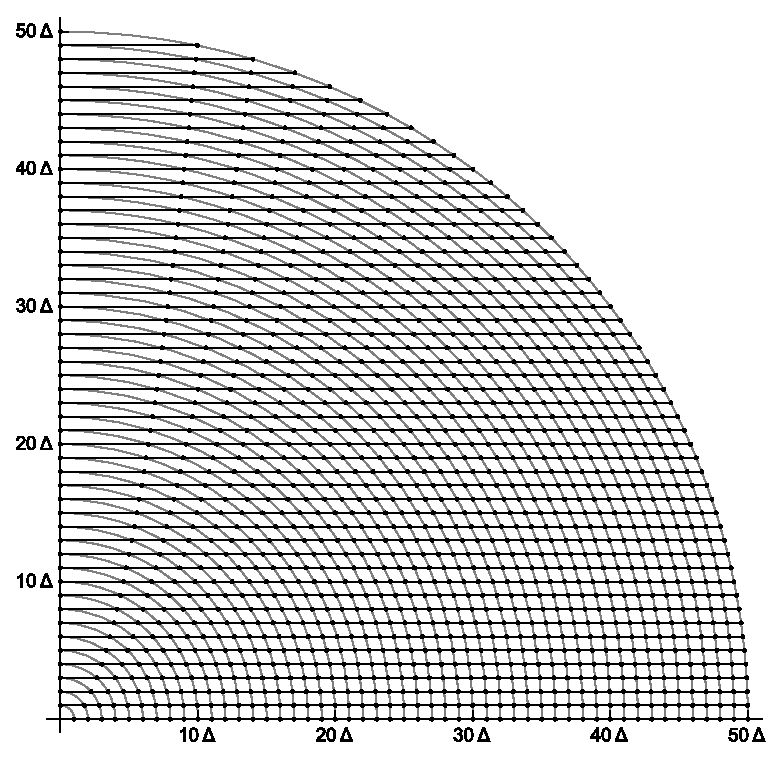
\includegraphics[ width = 2.25in ]{graphics/50_sectors.eps} \qquad
   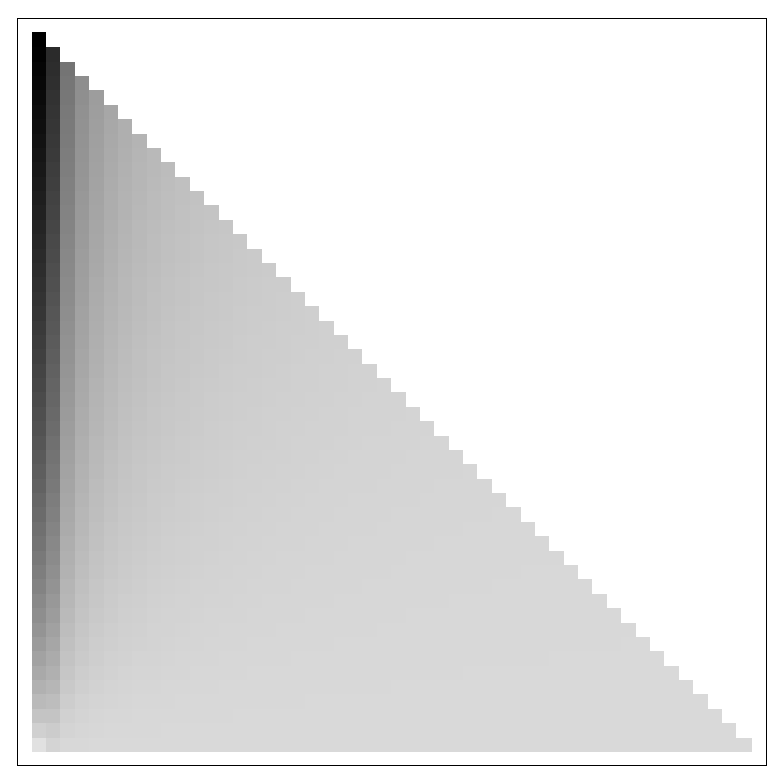
\includegraphics[ width = 2.25in ]{graphics/50_array_plot.eps} 
   \caption{A partition where $n=50$ showing the capsule sectors (left) and the $\B{}$ matrix (right).}
   \label{fig:n = 50}
\end{figure}

\begin{figure}[htbp] %  figure placement: here, top, bottom, or page
   \centering
   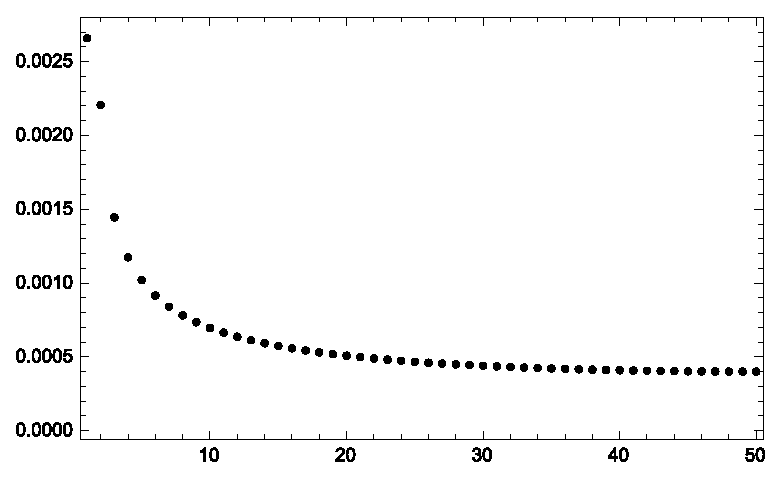
\includegraphics[ width = 4in ]{graphics/50_spectrum.eps}
   \caption{Eigenvalue spectrum.}
   \label{fig:n = 50 spectrum}
\end{figure}

\clearpage

%%  %%  %%  %%  %%  %%  %%  %%  %%  %%  %%  %%  %%  %%  %%  %%  %%  %%  %%  %%  %%

\Appendix

%     S   S   S   S   S   S   S   S   S   S   S   S   S   S   S   S   S   S   S   S
\section{Polynomials orthogonal over the unit disk}
We define the $\disk$, the closed unit disk, in three different coordinate systems: 
%%%
\begin{equation}
  \disc = 
    \begin{cases}
      \lst{z\in\cmplx{} \colon \abs{z} \le 1} \\
      \lst{\paren{ r, \theta }\in\real{2} \colon 0\le r \le 1, 0 \le \theta < 2\pi} \\
      \lst{\paren{ x, y }\in\real{2} \colon x^{2} + y^{2} \le 1}
    \end{cases}
    \label{eq:unit disk}
\end{equation}
%%%

%    SS  SS  SS  SS  SS  SS  SS  SS  SS  SS  SS  SS  SS  SS  SS  SS  SS  SS  SS  SS
\subsection{The set of Zernike}
Given non-negative integers $n$ for order and $m$ for angular frequency such that $n-m$ is even.
Recursion relationship: let the midpoint $\omega=\frac{1}{2}(n-m)$ and the average $\sigma=\frac{1}{2}(n+m)$ then: 
\begin{equation}
  R_n^m(r) = \sum_{j=0}^{\omega}{\paren{-1}^j\frac{(n-j)!}{j!\paren{\omega-j}!\paren{\sigma-j}!}r^{n-2j}}
  \label{eq:recursion}
\end{equation}

  % % % EQUATION
  \begin{equation}
    U_n^m(r,\theta) = R_n^{m}(r)e^{i m \theta}
  \end{equation}
  % %
\input{sections/"appendix a"/"tab Zernike polynomials"}  %  <  <  <  <  <  <  <  <  <  <  <  <  <  <  <  <
  
%   SSS SSS SSS SSS SSS SSS SSS SSS SSS SSS SSS SSS SSS SSS SSS SSS SSS SSS SSS SSS
\subsubsection{Change of basis}
The property that makes Zernike's set dominant in practical use is the ability to use exact affine transformations to monomial sets. This allows direct connection to Seidel aberrations on an order-by-order basis and it allows exact computation of amplitudes in discrete computation where the polynomials are no longer orthogonal.

For example, two functions are equivalent almost everywhere over the unit disk
  % % % EQUATION
  \begin{equation}
    \begin{split}
%
      P_{m}\paren{x_{1},x_{2}} 
        &= a_{00} + \paren{a_{10} x_{1} + a_{01} x_{2}} + \paren{a_{20} x_{1}^{2} + a_{11} x_{1}x_{2} + a_{02} x_{2}^{2}}, \\
%
      P_{Z}\paren{x_{1},x_{2}} 
        &= \alpha_{00} + \paren{\alpha_{10} Z_{1}^{1}\paren{x_{1},x_{2}} + \alpha_{01} Z_{1}^{-1}\paren{x_{1},x_{2}}} \\
        &+ \paren{\alpha_{20}  Z_{2}^{0}\paren{x_{1},x_{2}} + \alpha_{11}  Z_{2}^{2}\paren{x_{1},x_{2}} + \alpha_{02} Z_{2}^{-2}\paren{x_{1},x_{2}}}, 
%        
    \end{split}
  \end{equation}
  % % %

  % % % EQUATION
  \begin{equation}
    \mat{c}{ \alpha_{00} \\ \alpha_{10} \\ \alpha_{01} \\ \alpha_{20} \\ \alpha_{11} \\ \alpha_{02} }
      = 
    \mat{rrrrrr}{
 1 & 0 & 0 & -1 & 0 & 0 \\
 0 & 1 & 0 & 0 & 0 & 0 \\
 0 & 0 & 1 & 0 & 0 & 0 \\
 0 & 0 & 0 & 2 & 1 & 0 \\
 0 & 0 & 0 & 0 & 0 & 2 \\
 0 & 0 & 0 & 2 & -1 & 0
}^{-1}
    \mat{c}{ a_{00} \\ a_{10} \\ a_{01} \\ a_{20} \\ a_{11} \\ a_{02} }
  \end{equation}
  % % %

%   SSS SSS SSS SSS SSS SSS SSS SSS SSS SSS SSS SSS SSS SSS SSS SSS SSS SSS SSS SSS
\subsection{The set of Bhatia and Wolf}

%     S   S   S   S   S   S   S   S   S   S   S   S   S   S   S   S   S   S   S   S
\section{Emissivity and opacity}
While the radiative transport equation is elementary the components are quite intricate. The terms $j$ and $\alpha$ encode the interactions between the electrons, ions and radiation inside the capsule.

  % % % EQUATION
  \begin{equation}
    j(T,\rho) = a_{00} + \sum_{j=0}^{d}\sum_{k=0}^{d} a_{j-k,k}T^{j-k}\rho^{k}
  \end{equation}
  % % %

\input{sections/"appendix b"/"tab the emissivity"}  %  <  <  <  <  <  <  <  <  <  <  <  <  <
\input{sections/"appendix b"/"tab the opacity"}  %  <  <  <  <  <  <  <  <  <  <  <  <  <
\input{sections/"appendix b"/"tab surface fit quality"}   %  <  <  <  <  <  <  <  <  <  <  <  <  <
Figure \ref{tab:coeffs emis HeB I}: The error is shown in parentheses next to each amplitude. For example, the $a_{00} = 0.01861 \pm 0.000055$. The residual error in the $L_{\infty}$ norm is XX, in the $L_{2}$ norm XX.
\input{sections/"appendix b"/"tab amplitudes with errors"}   %  <  <  <  <  <  <  <  <  <  <  <  <  <
\clearpage


%     S   S   S   S   S   S   S   S   S   S   S   S   S   S   S   S   S   S   S   S
\begin{thebibliography}{1}

\bibitem{Bhatia} {\sc A.~B. Bhatia, and E. Wolf}, {\em On the circle polynomials of Zernike and related orthogonal sets}, Math. Proc. Cambridge Phil. Soc., 50 (1954), pp. 40-48.

\bibitem{Hummer} {\sc D.~G. Hummer, and G.~B. Rybicki},
{\em Radiative transfer in spherically symmetric systems. The conservative grey case}, Mon. Not. R. Astr. Soc., 152 (1971), pp. 1-19.

\bibitem{Trent} {\sc T.~T. Trent},
{\em A \ms theorem for $C(\overline{D})$}, Proc. Am. Math. Soc., 83 (1981), pp. 296-298.

\bibitem{Topa orthogonality} {\sc D.~M. Topa, and P.~F. Embid},
{\em Orthogonality, domains and linear independence}, some computation journal (in print).

\bibitem{Topa} {\sc D.~M. Topa, and P.~F. Embid},
{\em Surprising homotopies in the Zernike bases}, Applied Computational an Harmonic Analysis (in print).

\bibitem{Zernike} {\sc F. Zernike}, {\em Diffraction theory of the knife-edge test and its improved form, the phase-contrast method}, Mon. Not. R. astr. Soc., 94 (1934), 377-384.

\end{thebibliography}

\endinput %-------------------------------

\end{document}

%     S   S   S   S   S   S   S   S   S   S   S   S   S   S   S   S   S   S   S   S
%    SS  SS  SS  SS  SS  SS  SS  SS  SS  SS  SS  SS  SS  SS  SS  SS  SS  SS  SS  SS
%   SSS SSS SSS SSS SSS SSS SSS SSS SSS SSS SSS SSS SSS SSS SSS SSS SSS SSS SSS SSS
